\documentclass[12pt, twoside]{article}
\usepackage[letterpaper, margin=1in, headsep=0.5in]{geometry}
\usepackage[english]{babel}
\usepackage[utf8]{inputenc}
\usepackage{amsmath}
\usepackage{amsfonts}
\usepackage{amssymb}
\usepackage{tikz}
%\usetikzlibrary{quotes, angles}

\usepackage{graphicx}
\usepackage{enumitem}
\usepackage{multicol}

\usepackage{fancyhdr}
\pagestyle{fancy}
\fancyhf{}
\renewcommand{\headrulewidth}{0pt} % disable the underline of the header

\fancyhead[RE]{\thepage}
\fancyhead[RO]{\thepage \\ Name: \hspace{3cm}}
\fancyhead[L]{BECA / Dr. Huson / 10th Grade Geometry\\* Unit 7: Analytic Geometry Review\\14 February 2019}

\begin{document}
\subsubsection*{Do Now: Equations of circles on the coordinate plane}
  \begin{enumerate}

    \item On the set of axes below, graph the diameter of a circle $C$,  $\overline{AB}$ with $A(-2,5)$ and $B(4,-3)$.
      \begin{center} %4 quadrant regents grid
      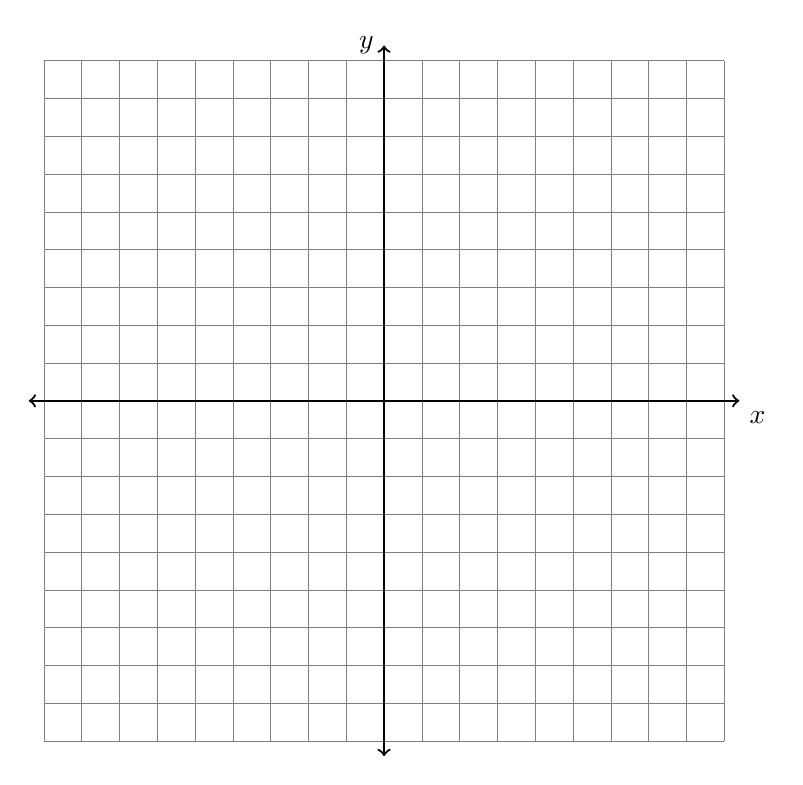
\begin{tikzpicture}[scale=.48]
        \draw [help lines] (-9,-9) grid (9,9);
        \draw [thick, <->] (-9.4,0) -- (9.4,0) node [below right] {$x$};
        \draw [thick, <->] (0,-9.4)--(0,9.4) node [left] {$y$};
        %\draw [thick] (-3,-3) node[below] {$A$}--
        %(5,1) node[right] {$B$}--
        %(6,8) node[left] {$C$}--
        %(-2,4) node[left] {$D$}--cycle;
        %\draw [fill] (5,0) circle [radius=0.1] node[above left] {$P$};
      \end{tikzpicture}
      \end{center}
      \begin{enumerate}
        \item Find the center of the circle, $C$, as an coordinate pair and mark it on the graph. \vspace{3cm}
        \item Find the radius of the circle. \vspace{3cm}
        \item Write down the equation of the circle in standard form.
      \end{enumerate}

\newpage


    \item Convert this quadratic function from vertex form to standard form ($f(x)=x^2+bx+c$) by expanding the squared term and simplifying.

        \[f(x) = (x-2)^2+4\]
    \vspace{3cm}

    \item In the quadratic function below, a constant value, $p$, ``completes the square".

    \[f(x) = x^2+14x+p-p\]

    \begin{enumerate}
      \item In the function, what are the values of the coefficients $a$ and $b$?
      \item What value of $p$ would complete the square?
      \item Rewrite the function $f$ in vertex form. \vspace{2cm}
      \item Write down the value of the vertex of the graph of $f$ as a coordinate pair.  \vspace{2cm}
    \end{enumerate}

    \item Given right $\triangle JKL$ with $\overline{JK} \perp \overline{KL}$, $m\angle J = 35^\circ$, and $JK=10$.\\
        \begin{multicols}{2}
          \raggedcolumns
          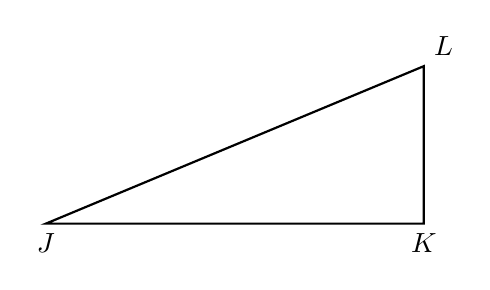
\begin{tikzpicture}[scale=0.4]
            \draw [thick]
            (0,0) node[below]{$J$}--
            (12,0)  node[below]{$K$}--
            (12,5) node[above right]{$L$}--cycle;
          \end{tikzpicture}
          \begin{enumerate}
            \item Find the length $KL$. \vspace{2cm}
            \item Find the length $JL$. \vspace{1cm}
          \end{enumerate}
    \end{multicols}


  \end{enumerate}

\newpage
\setcounter{page}{1}
\subsubsection*{Homework: Equations of circles on the coordinate plane}
  \begin{enumerate}


  \item On the set of axes below, graph the diameter of a circle $C$,  $\overline{AB}$ with $A(7,3)$ and $B(-5,-2)$.
    \begin{center} %4 quadrant regents grid
    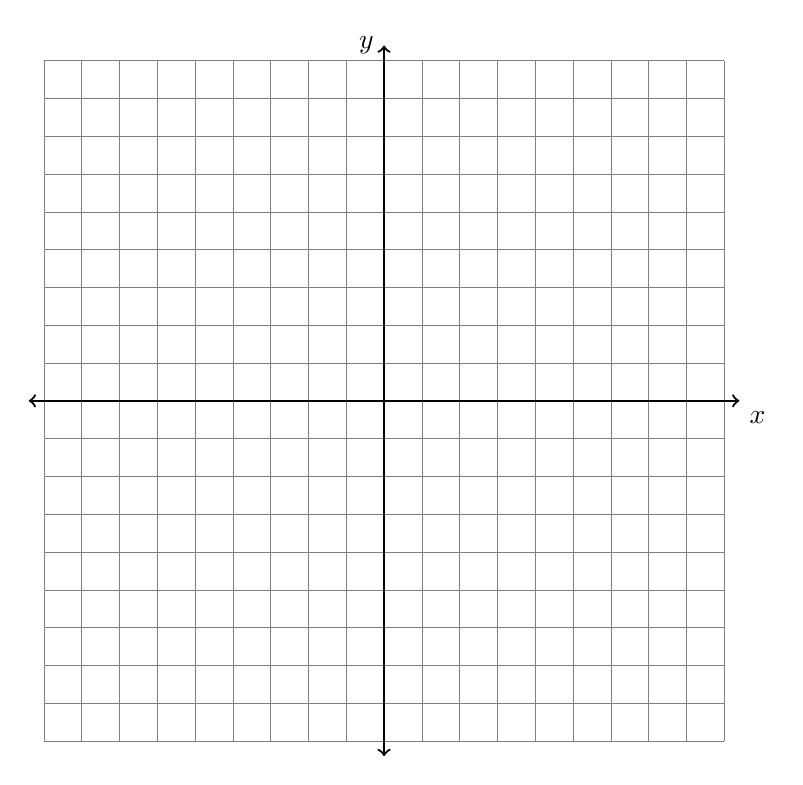
\begin{tikzpicture}[scale=.48]
      \draw [help lines] (-9,-9) grid (9,9);
      \draw [thick, <->] (-9.4,0) -- (9.4,0) node [below right] {$x$};
      \draw [thick, <->] (0,-9.4)--(0,9.4) node [left] {$y$};
      %\draw [thick] (-3,-3) node[below] {$A$}--
      %(5,1) node[right] {$B$}--
      %(6,8) node[left] {$C$}--
      %(-2,4) node[left] {$D$}--cycle;
      %\draw [fill] (5,0) circle [radius=0.1] node[above left] {$P$};
    \end{tikzpicture}
    \end{center}
    \begin{enumerate}
      \item Find the center of the circle, $C$, as an coordinate pair and mark it on the graph. \vspace{3cm}
      \item Find the radius of the circle. \vspace{3cm}
      \item Write down the equation of the circle in standard form.
    \end{enumerate}

\newpage

\item Write down the center and radius of each circle.
  \begin{enumerate}
    \begin{multicols}{2}
    \item   $(x-5)^2+(y-6)^2=25$ \vspace{2cm}
    \item   $(x+1)^2+(y+4)^2=8^2$
    \item   $(x-1)^2+y^2=36$ \vspace{2cm}
    \item   $(x+12)^2+(y-3)^2=3^2$
    \end{multicols}
  \end{enumerate}
  \vspace{2.5cm}

  \item In the quadratic function below, a constant value, $p$, ``completes the square".

  \[f(x) = x^2+8x+p-p\]

  \begin{enumerate}
    \item In the function, what are the values of the coefficients $a$ and $b$? \vspace{1cm}
    \item What value of $p$ would complete the square? \vspace{1cm}
    \item Rewrite the function $f$ in vertex form. \vspace{2cm}
    \item Write down the value of the vertex of the graph of $f$ as a coordinate pair.  \vspace{2cm}
  \end{enumerate}

  \end{enumerate}

  \end{document}
